
\documentclass[sigconf,nonacm]{acmart}
\usepackage{graphicx}
\usepackage{url}
\usepackage{todonotes}


%% up to 2 pages for distributing at SC19 and some other places to
%% have more number of answers

\def\Underline{\setbox0\hbox\bgroup\let\\\endUnderline}
\def\endUnderline{\vphantom{y}\egroup\smash{\underline{\box0}}\\}
\def\|{\verb|}
%
\long\def\comment#1{}
%

\begin{document}

\title{\textcolor{red}{Why are MPI users not using the state-of-the-art API?}\\
- An Interim Report for the MPI International Survey -}


\author{Atsushi Hori}
%\email{ahori@riken.jp}
\author{Takashi Ogura}
%\email{t-ogura@riken.jp}
\affiliation{\institution{R-CCS}}

\author{George Bosilca}
%\email{bosilca@icl.utk.edu}
\affiliation{\institution{The University of Tennessee}}

\author{Emmanuel Jeannot}
%\email{emmanuel.jeannot@inria.fr}
\affiliation{\institution{Inria}}

\maketitle

\section{Abstract}

The Message Passing Interface (MPI) is a critical part of the parallel computing
ecosystem, a driving force behind many of the high-performance computing (HPC) successes.
To maintain its relevance to the user community---and in particular to the HPC
community at large---we need to identify and understand the MPI users' expectations and concerns.

%
Existing studies on MPI uses are focused on a restricted target domain,
such as the Exascale Computing Project (ECP)~\cite{ECP} study conducted in 2017~\cite{osti_1462877} that focused
on MPI usage in the context of ECP applications; and/or those that are geographically
constrained to a single laboratory, funding agency or at best, country.
%In 2017, ECP~\cite{ECP} conducted a survey for MPI users in the ECP
%project to reveal how MPI would/should be integrated with ECP
%applications~\cite{osti_1462877}.
%
Such studies inspired us to conduct a larger study, not focused on HPC, but
targeting a wider audience and involving a larger spectrum of geographically
distinct users. Since MPI has been a widely used vehicle for high-performance
computing for decades, this larger-scale questionnaire survey would be
beneficial not only for deciding the future direction of MPI, but also the
feature differences of MPI users among countries and/or regions of the world.
% Our survey is both internation and targets novice to expert
% users, hoping to be a complement to the ECP survey.

This survey was conducted from February to June 2019, and at the time of
this writing has gathered more than 800 answers from 42 countries.
%
This first interim report, based the October 2019 results of the survey,
focuses on the MPI users communities awareness of MPI features.
% which MPI features MPI users know and which ones they do not.
%
This survey reveals the staggering fact that most MPI users use a small subset
of the MPI API, a subset that mostly avoids features introduced after MPI 2.2,
released in 2009, such as PMPI, dynamic process creation, and persistent
communications. Further, the survey reveals that many MPI users learn MPI
from the internet and/or some form of online documents, highlighting a shift in
the education of the target community.
%
These two outcomes seem to suggest that many MPI users failed to receive the
information about new MPI features because most internet sources are outdated
and lack support for them. It also suggests that one quick way to address this
is to provide the necessary education, possibly as part of the MPI Forum effort.

\section{Survey}

The points we kept in mind while we were designing the questions were: (a)
minimizing the number of questions, (b) making them easy to answer, and (c) avoiding ambiguity. The
questionnaire is implemented by using firstly Google Forms and later Microsoft
Forms, and distributed by sending emails to major mailing lists such as {\tt
hpc-announce}. All data, a Python program to analyze the answers, and all
reports published so far (including this one) are available on
GITHUB.\footnote{\url{https://github.com/bosilca/MPIsurvey.git}}

Table~\ref{tab:countries} shows the number of answers from top-10 countries. It
should be noted that the survey does not ask participants nationality, but
instead ask the most recent (last 5 years) country of employment.
% one of the questions asked where the participants worked most recently
% (within the last five years), not the nationality.
%In this report, the countries and regions (a set of countries) \todo{incomplete thought}
\vspace{-3mm}

\begin{table}[htb]%
\begin{center}%
\caption{\small Top 10 Countries of Participants}
\vspace{-3mm}
\label{tab:countries}%
\begin{tabular}{c|l|c}%
\hline%
Rank & Country & \# Participants \\%
\hline%
1 & Germany 	& 159 \\%
2 & France 	& 125 \\%
3 & Russia 	& 94 \\%
4 & UK 		& 64 \\%
5 & Japan 	& 63 \\%
6 & USA 		& 58 \\%
6 & Italy 		& 57 \\%
\hline
8 & Switzerland & 40 \\%
9 & South Korea & 27 \\%
10 & Austria 	& 26  \\%
\hline%
\multicolumn{3}{c}{42 countries, 838 participants} \\%
\end{tabular}%
\end{center}%
\vspace{-5mm}
\end{table}%

Most answers, around 80\%, come from research organizations
(universities and governmental research institutes).  We think this
diversity reflects not the characteristics of the countries, but
came from the biased questionnaire distribution.
Since this profile may bias the analysis of the results,
readers must keep this in mind when considering the  background.

\section{Some Results}

Table~\ref{tab:Q10-ans}, \ref{tab:Q14-ans}, \ref{tab:Q16-ans}, and
\ref{tab:Q17-ans} show the answer distribution for 4 questions out of
30. Note that the numbers in these tables reflect that these questions allow participants to choose multiple answers.
The actual number of participants who answered
each question is noted after the slash (/) of the total number
at the end of each table.

\begin{table*}[htb]%
%\footnotesize
\scriptsize
\begin{center}%
\begin{tabular}[t]{c}

\begin{minipage}{0.24\hsize}
\begin{center}%
\caption{\small How did you learn MPI?}%
\label{tab:Q10-ans}%
\begin{tabular}[t]{l|r}%
\hline%
Multiple Choice & \# Answers \\%
\hline%
Other lectures or tutorials & 436 (23.8\%) \\%
Articles found on Internet & 430 (23.4\%) \\%
MPI standard docs & 323 (17.6\%) \\%
Lecture(s) at school & 292 (15.9\%) \\%
Book(s) & 277 (15.1\%) \\%
Never learned MPI & 26 (1.4\%) \\%
other & 50 (2.7\%) \\%
\hline%
\multicolumn{1}{c}{total} & 1834 / 825 \\%
\hline%
\end{tabular}%
\end{center}%
\end{minipage}

\hspace{1mm}
\begin{minipage}{0.24\hsize}
\begin{center}%
\caption{\footnotesize How do you check MPI specifications when you are writing MPI programs?}%
\label{tab:Q14-ans}%
\begin{tabular}[t]{l|r}%
\hline%
Multiple Choice & \# Answers \\%
\hline%
Online docs. & 570 (30.1\%) \\%
Internet & 560 (29.6\%) \\%
MPI standard docs. & 424 (22.4\%) \\%
I ask colleagues & 185 (9.8\%) \\%
I read book(s) & 102 (5.4\%) \\%
I know all MPI routines & 43 (2.3\%) \\%
other & 11 (0.6\%) \\%
\hline%
\multicolumn{1}{c}{total} & 1895 /824 \\%
\hline%
\end{tabular}%
\end{center}%
\end{minipage}

\hspace{1mm}
\begin{minipage}{0.24\hsize}
\begin{center}
\caption{\small Which MPI features have you never heard of?}%
\label{tab:Q16-ans}%
\begin{tabular}[t]{l|r}%
\hline%
Multiple Choice & \# Answers \\%
\hline%
PMPI interface & 457 (24.5\%) \\%
Persistent comm. & 423 (22.7\%) \\%
Dynamic process creation & 380 (20.4\%) \\%
One-sided comm. & 128 (6.9\%) \\%
Communicator operations & 123 (6.6\%) \\%
MPI datatypes & 90 (4.8\%) \\%
Point-to-point comm. & 89 (4.8\%) \\%
Collective comm. & 86 (4.6\%) \\%
w/ OpenMP (multithread) & 86 (4.6\%) \\%
\hline%
\multicolumn{1}{c}{total} & 1,862 / 691 \\%
\hline%
\end{tabular}%
\end{center}%
\end{minipage}

\hspace{1mm}
\begin{minipage}{0.24\hsize}
\begin{center}
\caption{\footnotesize What aspects of the MPI standard do you use in your program in its current form?}%
\label{tab:Q17-ans}%
\begin{tabular}[t]{l|r}%
\hline%
Multiple Choice & \# Answers \\%
\hline%
Collective comm. & 729 (22.5\%) \\%
Point-to-point comm. & 701 (21.6\%) \\%
MPI datatypes & 512 (15.8\%) \\%
w/ OpenMP (multithread) & 472 (14.6\%) \\%
Communicator operations & 406 (12.5\%) \\%
One-sided comm. & 223 (6.9\%) \\%
PMPI interface & 66 (2.0\%) \\%
Persistent comm. & 61 (1.9\%) \\%
Dynamic process creation & 50 (1.5\%) \\%
other & 20 (0.6\%) \\%
\hline%
\multicolumn{1}{c}{total} & 3,240 / 813 \\%
\hline%
\end{tabular}%
\end{center}
\end{minipage}

\end{tabular}%
\end{center}%
\vspace{-3mm}
\end{table*}%

Table~\ref{tab:Q10-ans} shows the result of the question asking ``how
did you learn MPI.'' It is a bit surprising that 40\% (323/825) of
participants refer to the MPI standard. According to the original
data (omitted due to the space limit), one quarter of participants
learned MPI via the internet and/or online documents.

The result of the question asking ``How do you check MPI
specifications when writing MPI programs'' is shown in
Table~\ref{tab:Q14-ans}. More than half of participants refer to the
MPI standard. It is very natural for MPI users to check MPI
specification by referring the MPI standard more often than reading it
for learning. Most notably, the percentage of participants reading
online documents and/or referring the internet occupies 46\% (original
data).

Referring Table~\ref{tab:Q16-ans} and \ref{tab:Q17-ans}, the MPI
features can be categorized into two groups: well-known ones (P2P,
Collectives, and so on) and little-known ones (PMPI, Persistent and
Dynamic process). Surprisingly, this tendency is almost independent
from countries/regions of the participants.
(Figure \ref{fig:Q17} shows the percentages of answers over the
countries/regions having more than 50 answers.)

\comment{
Table~\ref{tab:Q16-ans} shows the answers of the question asking
``which MPI features have you never heard of?'' The answers of ``PMPI
interface,'' and ``Persistent communication,'' and ``Dynamic process
creation'' occupies almost 70\%.  The percentage of participants chose
one or some of them is 64\%.
Table~\ref{tab:Q17-ans} shows the answers of the question asking
``what aspects of the MPI standard do you use in your program in its
current form?'' This question asks the MPI features used by
participants, not if they know or not. Again, there are large gap
between those three features and the other features.
All those features was already standardized in MPI 2.2 which was
release in 2009. Despite the 10-year appearance, those features are
not well-known.
It is very interesting that the regional differences of the question
asking using MPI aspects over the
countries and regions having more
than 50 answers
(Table~\ref{tab:Q17-ans}) are very small as shown in
Figure~\ref{fig:Q17}.
}

\begin{figure}[htb]
\vspace{-2mm}
\begin{minipage}{0.8\hsize}
\begin{center}
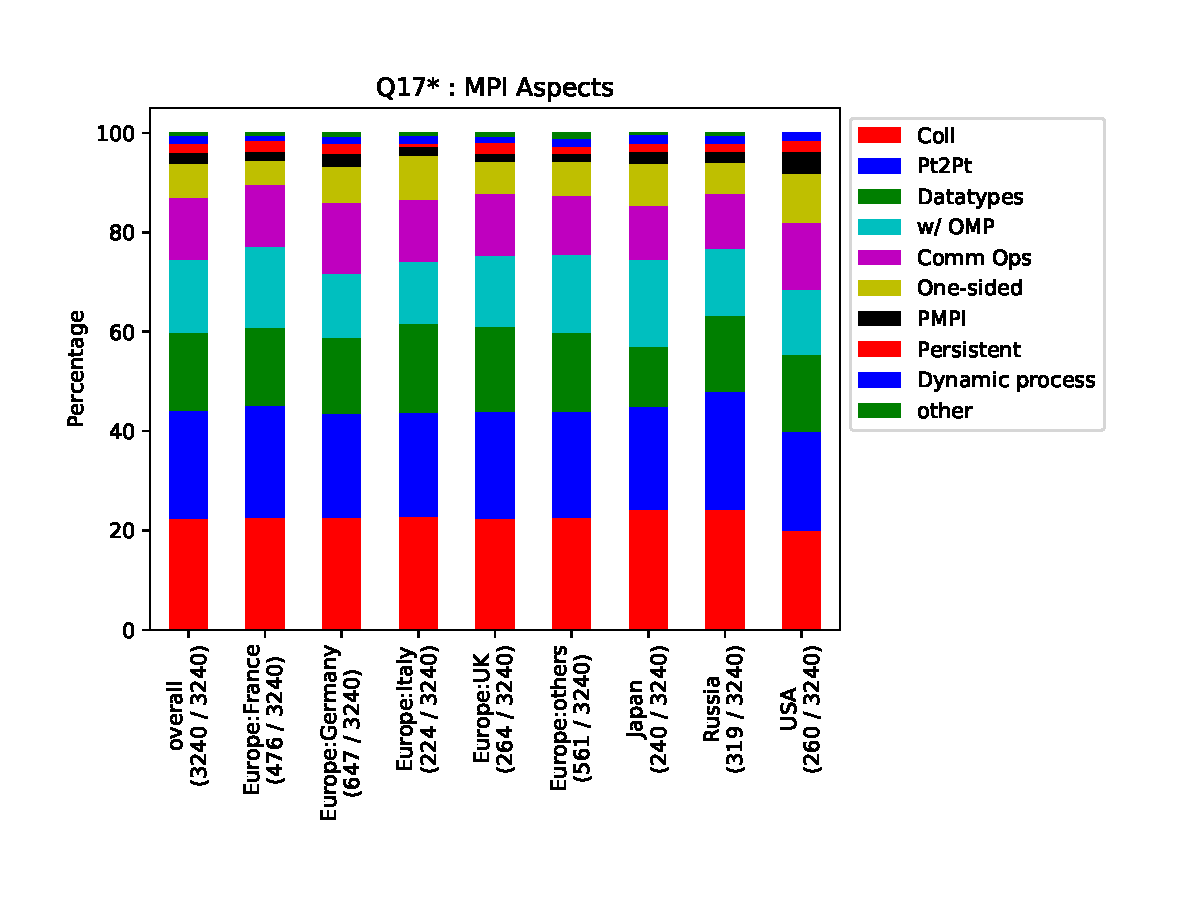
\includegraphics[width=7cm]{figs/Q17.pdf}
\vspace{-10mm}
\caption{What aspects of the MPI standard do you use in your program in its current form?}%
\label{fig:Q17}
\end{center}
\end{minipage}
\end{figure}

\comment{
On the question asking ``how did you learn MPI?,'' one quater of
participants answered ``internet,'' ``not learned,'' and ``other.'' Many
participants who chose ``other'' said ``learned from existing
code,''  ``learned by doing,'' etc.
\comment{Table~\ref{tab:Q14-ans} shows the result of asking ``how do you check
MPI specifications when you are writing MPI programs?'' }
When we ask ``how do you check
MPI specifications when you are writing MPI programs?,'' 45\% of
participants chose the answers only from ``Online Docs,''
``Internet,'' and ``Asking colleagues.''
30\% of participants chose ``too many routines,'' ``too complicated,''
and/or ``I have nobody to ask,'' when the question ``what are your
obstacles to mastering MPI?'' was given.
}
\comment{
\begin{table}[htb]%
\begin{center}%
\small
\caption{How do you check MPI specifications when you are writing MPI programs?}%
\label{tab:Q14-ans}%
\begin{tabular}{l|r}%
\hline%
Multiple Choice & \# Answers \\%
\hline%
{\small I read online documents (such as man pages).} & 570 (30.1\%) \\%
{\small I search the Internet} & 560 (29.6\%) \\%
{\small I read the MPI Standard document}  & 424 (22.4\%) \\%
I ask colleagues. & 185 (9.8\%) \\%
{\small I read book(s) (except the MPI standard).} & 102 (5.4\%) \\%
I know almost all MPI routines. & 43 (2.3\%) \\%
other & 11 (0.6\%) \\%
\hline%
\multicolumn{1}{c}{total} & 1,895 / 824 \\%
\hline%
\end{tabular}%
\end{center}%
\end{table}%
}

\section{MPI users do not use the state-of-the-art API}

Among the lesser-known MPI features, the persistent communication is
one of the important directions being discussed on the MPI Forum\cite{mpi-forum}.
The persistent communication can give implementors room for
optimizing not only P2P but also collective communication
performance.
All those little-known MPI features already appeared in MPI 2.2
released in 2009. Despite the 10-year appearance, those features
fail to be widely accepted.  Why?

One possible answer to this question may come from the survey results
asking participants ``how did you learn MPI''
(Table~\ref{tab:Q10-ans}) and ``how do you check
MPI specifications when you are writing MPI programs''
(Table~\ref{tab:Q14-ans}).
Here a significant number of participants refer to the internet
and/or online documents. These are handy and allow users to get
required information on the fly. However,
these online medias can only be retrieved by
search. To search something, a clue or some keywords must be given.
Say someone wants to search something he/she does not know; how can he/she
find the appropriate key words to obtain the right information?
This could be the responsibility of the information providers. For example,
there is no {\tt See Also} link from the man page of {\tt MPI\_Irecv}
to the corresponding persistent routines in many MPI implementations.

Contrastingly, traditional medias such as books, lectures, and tutorials can be
systematic and complete, but not handy.  Once you learned MPI via some
of those traditional medias, you may think that you already know
MPI. Unfortunately, the MPI standard is being updated by MPI Forum. It is
very hard to keep your MPI knowledge up-to-date, especially if MPI is not
your major concern.

The other point we noticed is that many people who chose the ``other''
answer to the question asking ``how did you learn MPI'' said
``reading existing code,'' ``learn by doing,'' ``reverse
engineering''(!),  and so on. Taking a look at existing code found on
internet might be the way of learning programing nowadays. However,
the underlying rationale of every MPI feature is never simpler than
any other sequential program. It is very likely that novice
programmers writing MPI programs in this way encounter difficulties.

\section{Summary and Future Work}

This large-scale international MPI survey reveals an uneven perception of the
MPI features, and a slow adoption of novel MPI capabilities.
%
Based on the survey, our hypothesis is that due to the large impact of online
sources, new features have a slow propagation time from the MPI standard to
the first page of a Google search. If this unevenness is not addressed by the MPI
Forum itself, most new MPI features will continue to have a slow adoption, and
their usefulness will be limited to only niche communities.
% As the result of conducting an international, large-scale MPI survey,
% it is revealed that the uneven perception in the MPI features.
% Our hypothesis of this unevenness based on the survey results
% is that many MPI users nowadays learn MPI directly from online sources. If this
% unevenness will not be fixed then the new MPI features
% introduced by MPI Forum might also have a slow adoption by the user community.
% This can ruin the large effort of MPI Forum.

As contributions from some countries known to be early and eager HPC adopters
are below the necessary threshold to make accurate and constructive
conclusions, we decided to publish intermediary results and leave the
survey open until we got a representative number of answers from most countries.
%
Readers are strongly encouraged to visit one of the URLs in the QR codes below.
% We are trying to increase the number of participants from other
% countries which are aggressive in HPC.
% If readers are interested in participating this survey,
% visit one (not both) of the URLs in
% Figure~\ref{fig:qrcodes}.

\begin{figure}[htb]
\begin{center}

\includegraphics[width=7cm]{figs/QR-codes.pdf}
\vspace{-3mm}
\caption{QR codes for participating this survey}
\label{fig:qrcodes}
\end{center}
\vspace{-5mm}
\end{figure}

\section*{Acknowledgments}
{\small
We thank to those who participated in this survey and those who
helped us to distribute the survey to their local communities.
This research is partially supported by the
NCSA-Inria-ANL-BSC-JSC-Riken-UTK Joint-Laboratory for Extreme Scale
Computing\cite{JLESC}.
}
\bibliographystyle{acm}
\bibliography{../ref}

\end{document}
